% !TeX encoding = UTF-8
% !TeX program = pdflatex
% !TeX spellcheck = it_IT

\documentclass[LaM,binding=0.6cm]{sapthesis}

\usepackage{microtype}
\usepackage[english]{babel}
\usepackage[utf8]{inputenx}
\usepackage{listings}
\usepackage{setspace}
\onehalfspacing
\usepackage{multirow}

\usepackage{hyperref}
\usepackage{qtree}
\hypersetup{pdftitle={},pdfauthor={Sara Di Bartolomeo}}

% Remove in a normal thesis
\usepackage{lipsum}
\usepackage{curve2e}
\definecolor{gray}{gray}{0.4}
\newcommand{\bs}{\textbackslash}

% Commands for the titlepage
\title{Ontology extraction and population \\ from user-generated text on online marketplaces}
\author{Sara Di Bartolomeo}
\IDnumber{1494990}
\course{Ingegneria Informatica}
\courseorganizer{Ingegneria dell'Informazione, Informatica e Statistica}
\AcademicYear{2016/2017}
\copyyear{2017}
\advisor{Prof. Riccardo Rosati}
\coadvisor{Dr. Nome Cognome}
\authoremail{dibartolomeo.sara@gmail.com}

\examdate{16 April 2013}
\examiner{Prof. Nome Cognome}
\examiner{Prof. Nome Cognome}
\examiner{Dr. Nome Cognome}
\versiondate{\today}



\begin{document}

\frontmatter

\maketitle

\dedication{Dedicato a\\ }

\begin{abstract}
%This document is an example which shows the main features of
%the \LaTeXe\ class \texttt{sapthesis.cls} developed by Francesco Biccari with the help of GuIT (Gruppo Utilizzatori Italiani di \TeX).
\end{abstract}

\begin{acknowledgments}
I would like to thank the whole Dipartimento di Ingegneria Informatica, Automatica e Gestionale at Sapienza. 
From what I experienced, the department aggregates a great deal of brilliant and passionate students and professors, from which I had the opportunity to learn the proudness in dedication and discipline, the love for the subjects, the long lasting satisfaction in pursuing achievements.
The years I have spent in this building forged me into an Engineer, with a sharp attention for details and a deep rooted thirst for knowledge.
\\
\\
Specifically, I would like to thank professor Riccardo Rosati, who has been my thesis advisor, who trusted my ideas and wisely guided me through the process of shaping them into a Master's thesis.
\\
\\
I would also like to thank each one of my colleagues, as many of them have been role models and figures of guidance to me. Matteo, Alessandro, Lorenzo, Alessio, Gabriele [etc]. Along with them, I want to mention a couple of colleagues from Codemotion, Massimo and Bruno, who made me really understand that creativity and technology weren't mutually exclusive concepts, and with whom I had a productive friendship that made me grow up []
\\ 
\\
Lastly, I want to thank the single person who has been, at the same time, a loving partner, a perfect teammate, and a best friend. 
Giorgio, who has been at my side through all the difficulties I had to face. 
\\

\end{acknowledgments}

\tableofcontents

\mainmatter

\chapter{Introduction}
 In recent years, the shopping habits of the general public have been changing considerably: more and more people are choosing to use online marketplaces for their purchases. This form of shopping platform has introduced several advantages: users have access to a much bigger selection of products, barriers that would otherwise have prevented access to the market to smaller sellers have been broken down.

 Nevertheless, these advantages are balanced by other downsides. As an example, judjing the quality and features of an item is a more complex task, as an user will only have access to photos and textual descriptions of the item.

 In this context, a trust-based system between multiple users has gained more and more relevance: reviews and reputation. The judgement of a buyer will be substantially affected by other users' reviews, as well as a level of trustworthyness assigned to sellers by other users.

 We have to take into account that reviews represent a relevant strategic resource to sellers.
 Making an user able to gain knowledge about the quality, purpose and details of an item is a problem that concerns not only the users, but also the sellers. Indeed, a number of good reviews may be the deciding factor for a successful sale. 

 [sellers buying reviews] \\
 quotes on trust system

 \bigskip

 Since reviews are so relevant, they have been the object of a series of studies. They are, infact, made of unstructured informations about a product: the data they contain, if succesfully extracted, may help in identifying precisely the features of a product. 

 The overwhelming amount of informations contained in reviews makes them difficult to consider in every detail for a human reader. 

 If we consider the scale on which the informations we obtain becomes significative, though, we notice that an automatized system for extracting information from text is needed. 

 The project presented in this thesis is aimed at extracting and structuring the information contained in user generated content regarding products on online marketplaces. 



 Natural Language Processing is the field that studies the interpretation, from an algorithmic point of view, of phrases in commonly written/spoken languages. Thanks to advancements in this field, we are able 




 %As data becomes more and more important, the idea of making use of the wealth of text produced by internet users in the form of comments or reviews is now widespread. \\

\chapter{Related works}

In 2012, S.Z. Haider \cite{haider_ontology_2012} published a case study in which he used reviews from Amazon to populate an ontology. His approach used a pre-made ontology about mobile phones, and applied sentiment analysis to the Amazon reviews of three specific items (three mobile phones) to understand the opinion of the public about the qualities of the items that were being analyzed.

Biemann \cite{biemann_ontology_2005} published in 2005 a survey of methods to study the different approaches at extracting data from unstructured text in order to build an ontology. 

Julian McAuley and Alex Yang \cite{mcauley_addressing_2016} used an approach based on machine learning to classify questions and answers in the Questions/Answers section of Amazon.
\\

The purpose of this thesis is to build on the aforementioned works to:
\begin{itemize}
	\item include information from Questions/Answers sections as well as reviews
	\item include a much bigger range of products and categories of products
	\item  extract the structure of the ontology from the data
\end{itemize}

\chapter{Collecting Data}

Modern online marketplaces often offer customers the ability to give feedback to the vendors, often in the form of reviews. Recently, some platforms also started to insert question/answer forms, in order to let the users be able to formulate questions about a product, and have other users or the seller respond to their inquiries about the product. \\

Feedback is given by the users in the form of:
\begin{itemize}
	\item Numerical score (i.e. 1 to 5 stars)
	\item Reviews
	\item Questions and Answers
\end{itemize}

Although the first value is very easy to be semantically represented, the latter ones aren't so straightforward. They are, infact, expressed in natural language, and their analysis will be the focus of the following chapters. \\

The first step of the project is, thus, the collection of data. 

\section{Amazon}

The main focus of the project is extracting data from the biggest marketplace as of today, namely, Amazon. As stated in an article by Business Insider \cite{intelligence_amazon_nodate}, Amazon is accountable for 43\% of online sales in the US in 2016. \\

TODO: insert more data about amazon, explain why amazon is important

\begin{figure}
\centering
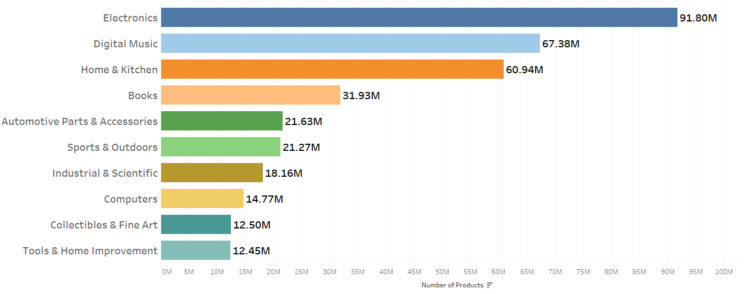
\includegraphics[width=0.7\textwidth]{pictures/prod_types.png}\\[3ex]
\caption{a comparison between different product categories on Amazon}
\label{fig:prod-types}
\end{figure}

\section{The challenges}

\subsection{Amazon API}
Amazon offers an API that makes available some of the information I wanted to examine. Unfortunately, not the request limits imposed to API users nor the information made available were useful for the purpose of this project. \\
Indeed, on 8 November 2010 Amazon removed the possibility to retrieve reviews from their API, returning now an URL to an IFrame containing just the first three reviews. The reason behind the removal of this feature were never explained by Amazon, and it has been discussed that the huge amount of data represented by written feedback is now considered a valuable resource that Amazon wants to protect. \\
Offering the first three reviews in an IFrame is intended for sellers to showcase on their website some Amazon reviews about their products, but I needed much more than just three reviews per product. The nature of the IFrame DOM element makes it difficult to deal with for accessing its contents, and makes the process of retrieving clean review content similar to the process of scraping a web page. \\


\section{Scraping}

Scraping is a technique for extracting data from a website via a software program. Scraper programs simulate human behaviour in accessing the content in webpages, with the purpose of collecting and transforming unstructured data, often found inside the HTML code of webpages, in metadata useful for being memorized, manipulated and analyzed locally.

A scraper program will access the content on a page directly through the HTTP protocol. A page is first downloaded through an HTTP GET request, in the same way in which a browser would request a page for visualizing it. The web server at the requested address will respond with the HTML code used by the browser to visually render the page. Instead of rendering it, a scraper will parse the code of the page to find patterns and references for purposeful data in the HTML. An example of this is contact scraping: a scraper is useful in finding all the email addresses in a page.

Commonly, scraping is done on a huge number of pages at the same time, and is therefore deeply linked with web crawling, that is the technique of navigating through a series of links to obtain a huge number of pages.

In addition to a number of challenges directly involved in the process, some websites will try to prevent this practice through various techniques, like IP blacklisting, CAPTCHAs, A/B testing and obfuscation of the content.

\subsection{Scraping a single page}

Scraping a single web page is performed in the following steps:

\begin{enumerate}
	\item An HTTP GET request is used to download the HTML code of the page that is being analyzed. The response, if the request was successfull, is HTML plain text.
	\item The response is then parsed to identify HTML components.
	\item Thanks to the tree-like structure of HTML elements in a page, each component is stored in a tree shaped data structure, called parsetree.
	\item The parsetree is searched according to several criteria (an example may be regular expression matching) to extract relevant data.  
\end{enumerate}

\begin{lstlisting}[language=HTML]
HTTP/1.1 404 Not Found
Date: Sun, 18 Oct 2012 10:36:20 GMT
Server: Apache/2.2.14 (Win32)
Content-Length: 230
Connection: Closed
Content-Type: text/html; charset=iso-8859-1
<html>
<head>
   <title>404 Not Found</title>
</head>
<body>
   <h1>Not Found</h1>
   <p>The requested URL was not found on this server.</p>
</body>
</html>
\end{lstlisting}
\label{code:example_html}

\begin{figure}
\Tree [.<html> [.<head> [.<title> {404 Not Found} ] ] [.<body> [.<h1> {Not Found} ] [.<p> {The requested URL was \\ not found on this server.} ] ] ]
\caption{The parsetree generated from \ref{code:example_html}}
\end{figure}

For the purpose of parsing, storing and accessing the result of the request, I used a python library designed to ease this task, BeautifulSoup \cite{noauthor_beautiful_nodate}. Processing the page in this way allows me to navigate HTML easily and query the contents. \\

In the code example above, at \ref{code:example_html}, retrieving the title of the received page would be written like this:
\begin{lstlisting}[language=Python]
BeautifulSoup bs = BeautifulSoup(res, 'html.parser')
title = bs.find('title').text
\end{lstlisting}
This code would perform a search on the document's parsetree, then extract what is contained in the tag \texttt{<title>}.


Real world html pages are much more complex than this, usually containing thousands of tags, and are often dynamically generated, thus require fine scraping criteria. The procedure used needs to be able to adapt to slight modifications in the page structure and contents.

As you can see in \ref{fig:amazon-page}, the structure of a standard product page on Amazon is convoluted, and identifying the parts that contain relevant information via code may not be straightforward. 

\begin{figure}
\centering
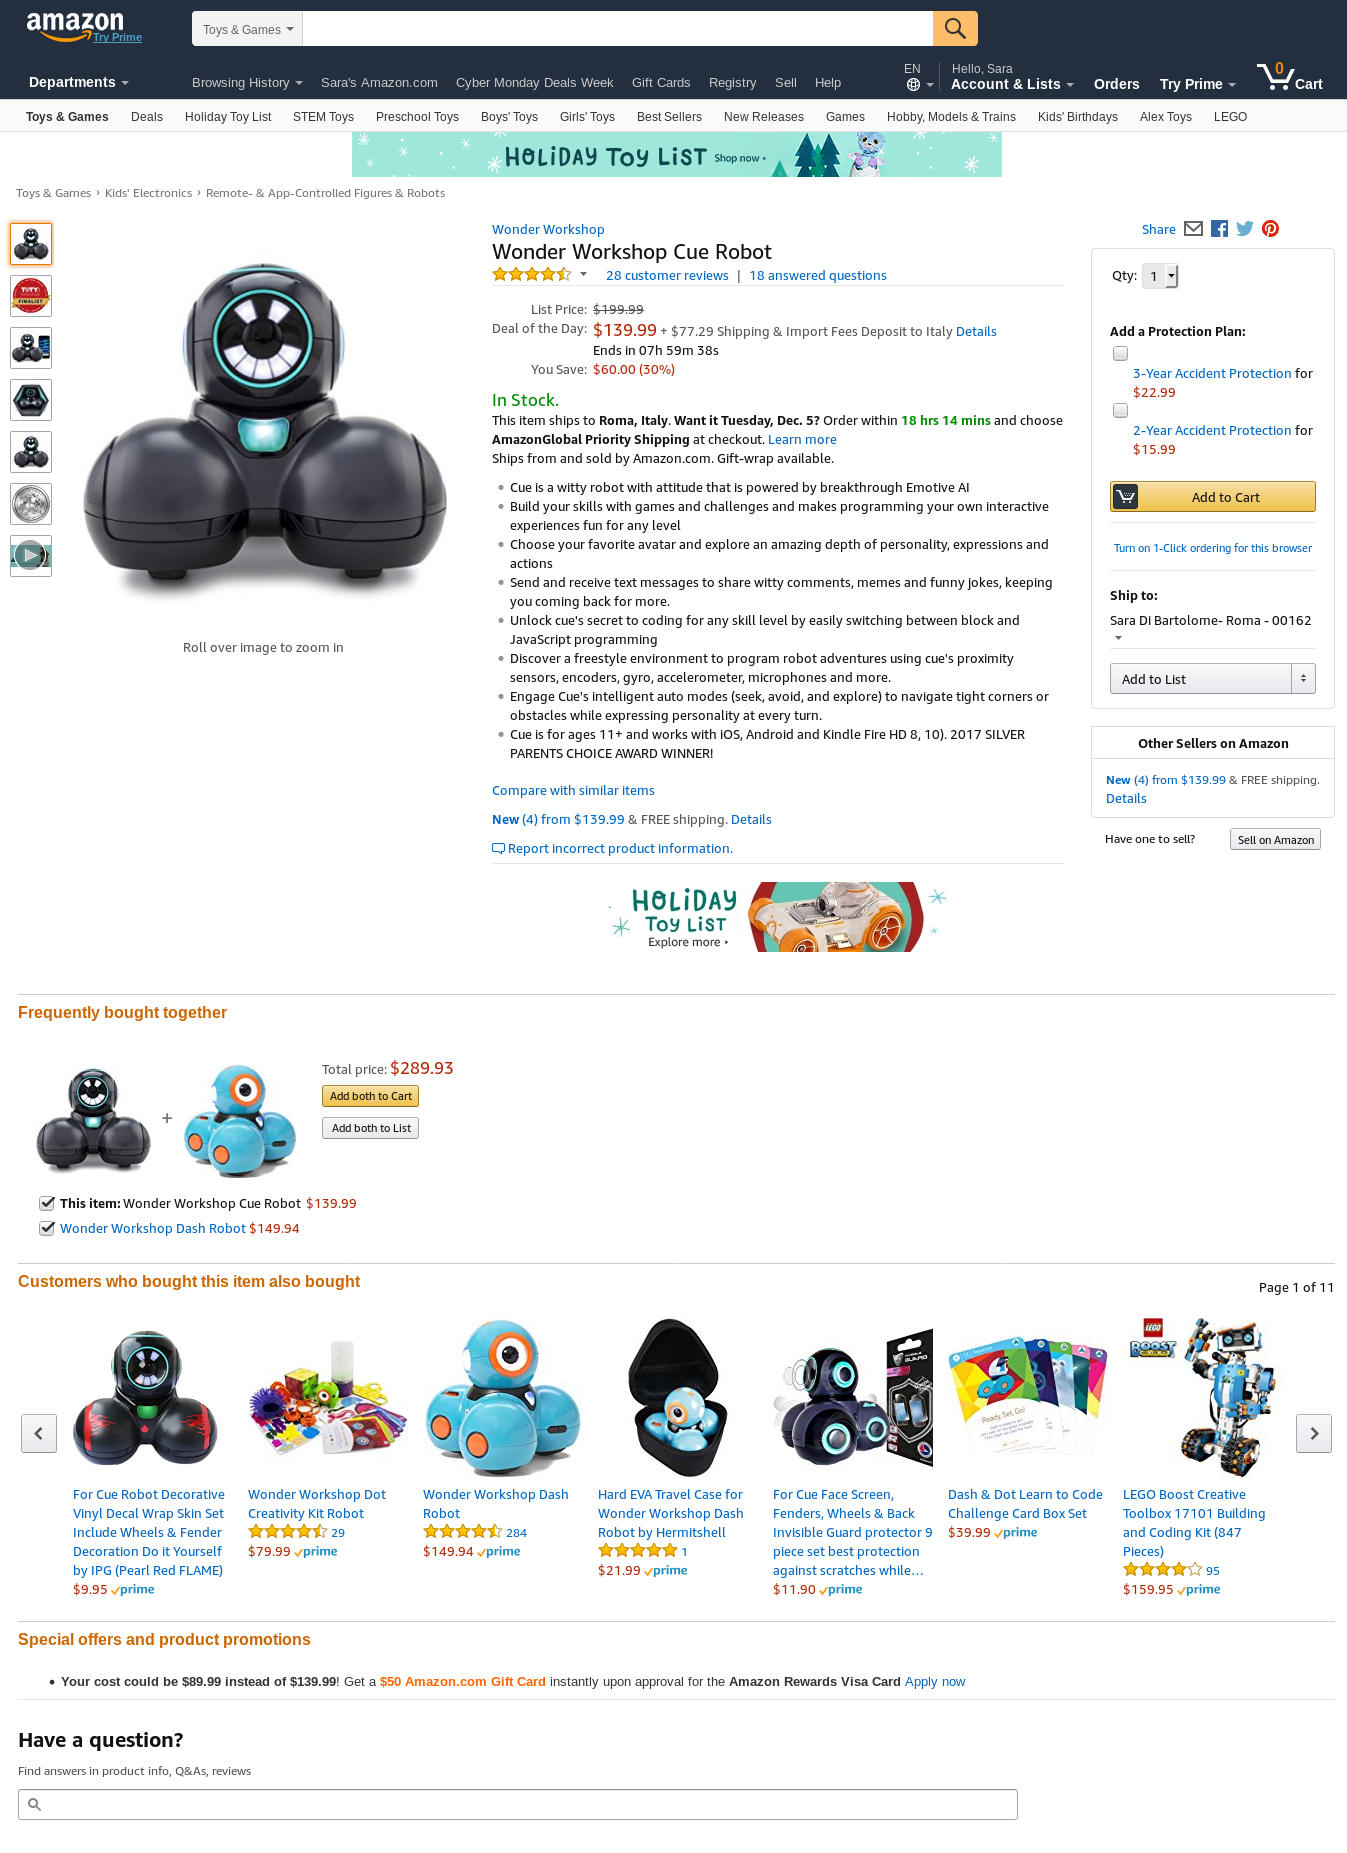
\includegraphics[width=0.7\textwidth]{pictures/amazon_page.png}\\[3ex]
\caption{a product page on amazon}
\label{fig:amazon-page}
\end{figure}


\subsection{Dynamic pages}

The modern web is comprised of a huge amount of content that is purposefully tailored for the user's needs and desires. In particular, when an HTTP request is made to a server, the server may respond with content specifically tailored for the particular user who made the request.

Think of facebook: each user sees the same website at the same address in a unique way, depending on the user's account, the cookies he has stored in its website, the times and types of content that the user's friends posted.

This may happen in the case of:

\begin{itemize}
	\item visual elements: a small screen with scarce resolution won't have the ability to display pictures as large and detailed as those needed on a Retina display. For this reason, websites often choose to serve smaller resolution pictures to devices with less displaying capabilities. The visual differences may also affect the way the website's UI is intended, to reflect the way of interacting with the requesting devices: mobile browsers used via touch input often require a different interface design than the one used for their desktop version.
	\item content: [example]
\end{itemize}

Therefore, a web server does not store a single web page for each 

\section{Scraping on a larger scale}

Scraping a large quantity of content introduces several challenges that I had to overcome. 

\subsection{Identifying bottlenecks}

\subsection{Multithreading}

\section{Tampering requests}

\subsection{Proxies}
\subsection{Crafting user agents}


\section{amazon-scraper}
\texttt{amazon-scraper} is the name I gave to the software I wrote. In \ref{fig:amazon-scraper}

\texttt{amazon-scraper} features:
\begin{itemize}
	\item 
	\item
\end{itemize}

\begin{figure}
\centering
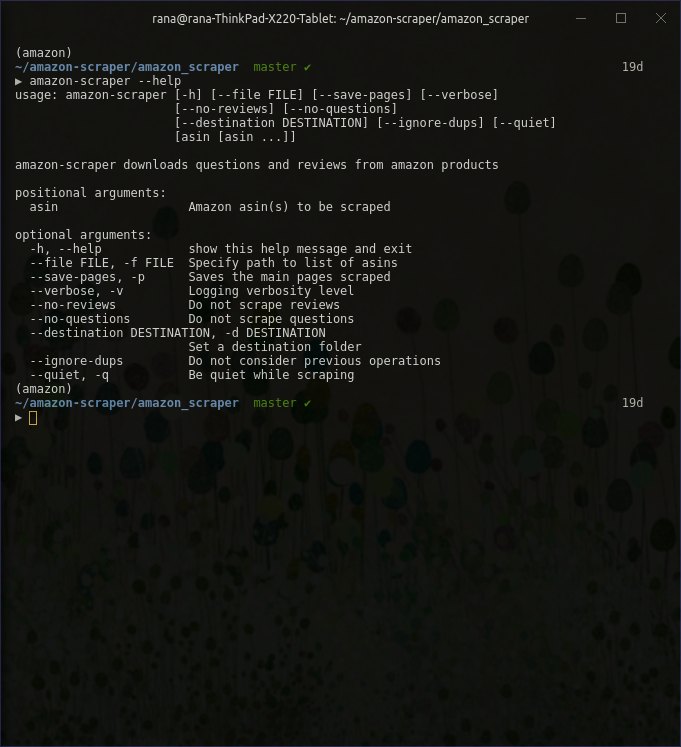
\includegraphics[width=0.7\textwidth]{pictures/1.png}\\[3ex]
\caption{\texttt{amazon-scraper} usage}
\label{fig:amazon-scraper}
\end{figure}

\section{Shape of the collected data}

\chapter{Processing the information}

Once enough data has been gathered, we can proceed with the language analysis part.
The intent of this analysis is to extract meaningful information from text. User generated text on product pages can infact contain relevant details about a product, that may or may not be specified in the seller's description of the same product. 

The reasons for a missing detail in the seller-provided [?] description may be several:
\begin{itemize}
	\item The seller didn't consider the detail relevant, but discussion about the detail present in the product's comments proves that clients consider the detail important
	\item The seller forgot to include the detail
	\item The seller didn't realize that his product had a particular characteristic
	\item The seller lied about a characteristic of his product
\end{itemize}

The characteristics listed above define a knowledge about the product that may be considered useful for a client to judge a product, but may not be easily understood. Moreover, these characteristics are relevant in our intent of building an ontology of products.

[add content here]

\section{Natural language processing}

Natural Language Processing is the process of programmatically treating information written in natural language, that is in this case American English. 

Natural language contains data, but that data is not easily usable by a computer program. A phrase like

\begin{quote}
This tablet costs 279\$
\end{quote}

clearly contains a relevant information: the price of an item we may be interested in, clearly underlined by the fact that the string contains a number. Nevertheless, our human brain is wired to understand that the number represents a price, but the same is not a straightforward process for a computer program. The process is made more difficult by the underlying ambiguity of the human language. 

The process of analyzing a string is performed in four different stages:
\begin{itemize}
	\item Splitting the string in sentences and words, namely \textit{tokens}
	\item Assigning each chunk (or word) a part-of-speech tag
	\item Arranging the tokens in a syntactical structure (a \textit{parsetree})
	\item Assignign to the structure a semantical meaning
\end{itemize}

[decision trees for tagging vs machine learning techniques]

To perform these tasks (for example, part-of-speech tagging), we rely on machine learning techinques to learn from a large \textit{corpora} \footnote{A copora is a large collection of documents with human-made annotations} how certain words in certain positions are intended.

The machine learning approach is much more versatile because it is able to manage unfamiliar structures - that is, structures of the phrase that were not present in the original dataset, but can be derived from similar entries.

\subsection{Pattern recognition in strings}

\subsection{Named entity recognition}

[explain better how named entity recognition works]

An important task in this project was the extraction of relevant entities from the sentences written by the users.

For this purpose, a python library, \texttt{spacy}, has been used. \texttt{spacy} features a default model that maps entities to []

An example of Named Entity Recognition performed on a simple phrase:
\begin{quote}
Linus Benedict Torvalds \textsuperscript{Person} (born December 28, 1969 \textsuperscript{Date}) is a Finnish \textsuperscript{NORP} software engineer who is the creator, and for a long time, principal developer of the Linux \textsuperscript{ORG} kernel.
\end{quote}

It can easily be noticed that this sentence contains a lot of information: named entity recognition can recognize where the relevant data is, and what kind of data type it is.

\subsection{Language use differences in reviews and questions}

After having collected enough data, it became apparent that there were relevant differences in language usage in Q/A and reviews. Questions, indeed, tend to be much shorter, use a simpler language and are much more straightforward than reviews. Although very short reviews can be found when dealing with a very diverse set of user generated content, they usually talk about multiple features of a product, while questions and answers usually address just one information. The structure of a sentence is also evidently different.

For this reason, I deemed appropriate to separate the methods in which Q/A and reviews are treated in the analysis process.

\begin{figure}
\centering
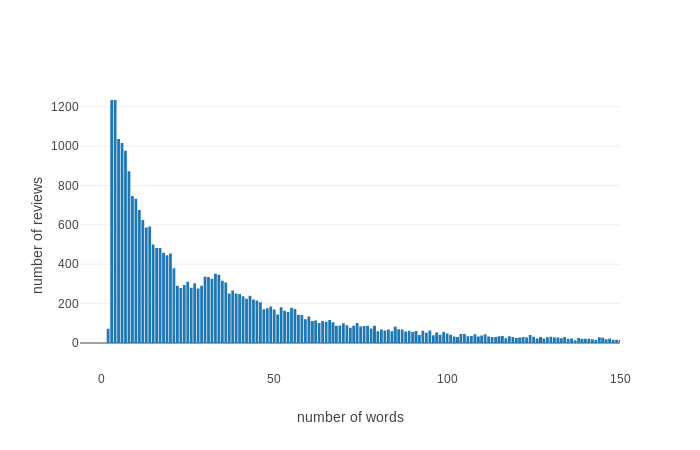
\includegraphics[width=0.8\textwidth]{pictures/reviews_freq_dist.png}\\[3ex]
\caption{Frequency distribution of the number of words used in reviews}
\label{fig:rev-freq-dist}
\end{figure}

\begin{figure}
\centering
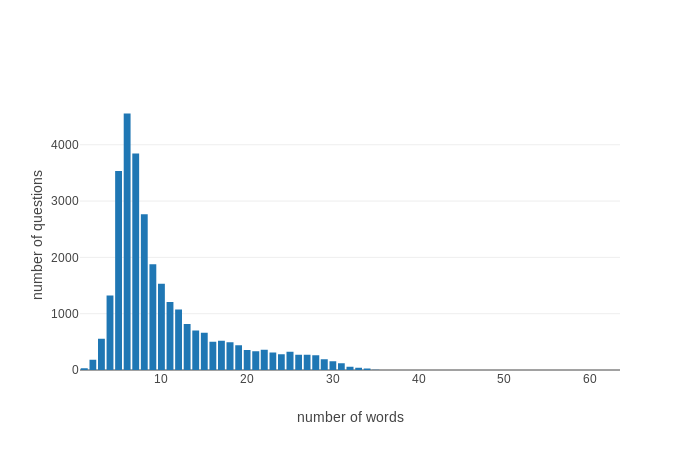
\includegraphics[width=0.8\textwidth]{pictures/quest_freq_dist.png}\\[3ex]
\caption{Frequency distribution of the number of words used in questions/answers}
\label{fig:quest-freq-dist}
\end{figure}

In \ref{fig:quest-freq-dist} and \ref{fig:rev-freq-dist}, the frequency distribution of the number of words used in both reviews and questions/answers is shown. It can clearly be seen that it is much more common for questions to employ much less words, while reviews are more verbose.

Another indicator of a more complex use of the language in reviews is [variance in frequency distribution of words]

[insert average question length for type of question]
[insert word frequency distribution for each category]

\section{Questions and Answers}

\subsection{Open-ended questions and closed-ended questions}

Questions about a product on a online marketplace can be open-ended or closed-ended. The affiliation of each question to one of these categories entails major differences in how information is expressed. \\

A \textbf{closed-ended} question is a question that accepts 'yes' or 'no' as answer. An example of a closed-ended question is:
\begin{quote}
\textbf{Question:} Does this phone have a camera? \\
\textbf{Answer:} Yes.
\end{quote} 

An \textbf{open-ended} question is, instead, a question that expects a more complex answer, such as a list, an explanation, a description. An example of an open-ended question is:
\begin{quote}
\textbf{Question:} What features does this phone have? \\
\textbf{Answer:} A camera, two sim slots and a headphone jack.
\end{quote}

As you can see, information is expressed in a very straightforward way in closed-ended questions. If we, through natural language processing, manage to understand the object of the question, the answer is just a boolean value representing if the analyzed product corresponds to the requested quality or not.

\subsubsection{Classifying the questions}
Based on the work of [insert link], I used a simple Naive Bayes classifier to discern closed-ended from open-ended questions.
The classifier has been trained on a pre-labeled dataset of [N] questions and answers. The labels were "open" or "Y/N".

\subsubsection{Classifying the answers}
In the case of closed-ended questions, I analyzed the answers.
The answers may be as simple as a "Yes" or "No", and in this situation the outcome is straightforward, but it is not always the case.
Positive answers may appear in forms similar to:
\begin{quote}
\textbf{Question:} Does it work in Argentina? \\
\textbf{Answer:} It does work very well in Argentina.

\textbf{Question:} Does it work in Argentina? \\
\textbf{Answer:} Absolutely.

\textbf{Question:} Does it work in Argentina? \\
\textbf{Answer:} I think it does.
\end{quote}
These are positive forms, but do not include the term "Yes". \\

Another detail to take into account is the possibility for a user to answer with an unclear or undefined answer. For this purpose, when classifying the answers, we consider a third "Unknown" label.
Answers along the lines of:

\begin{quote}
\textbf{Answer:} I don't know.
\textbf{Answer:} I'm not sure.
\end{quote}

or other unclear answers are considered Unknown answers.

\subsection{Detecting the object of a question}
[better]
Named entities are definite noun phrases that refer to specific types of individuals, such as organizations, persons, dates, and so on. 5.1 lists some of the more commonly used types of NEs. These should be self-explanatory, except for "Facility": human-made artifacts in the domains of architecture and civil engineering; and "GPE": geo-political entities such as city, state/province, and country.



\begin{center}
\begin{tabular}{ c c }
ORGANIZATION &	Georgia-Pacific Corp., WHO \\
PERSON 	& Eddy Bonte, President Obama \\
LOCATION &	Murray River, Mount Everest\\
DATE &	June, 2008-06-29\\
TIME &	two fifty a m, 1:30 p.m.\\
MONEY &	175 million Canadian Dollars, GBP 10.40\\
PERCENT &	twenty pct, 18.75\% \\
FACILITY &	Washington Monument, Stonehenge\\
GPE &	South East Asia, Midlothian \\
\end{tabular}
\end{center}

The goal of a named entity recognition (NER) system is to identify all textual mentions of the named entities. This can be broken down into two sub-tasks: identifying the boundaries of the NE, and identifying its type. While named entity recognition is frequently a prelude to identifying relations in Information Extraction, it can also contribute to other tasks. For example, in Question Answering (QA), we try to improve the precision of Information Retrieval by recovering not whole pages, but just those parts which contain an answer to the user's question. Most QA systems take the documents returned by standard Information Retrieval, and then attempt to isolate the minimal text snippet in the document containing the answer. Now suppose the question was Who was the first President of the US?, and one of the documents that was retrieved contained the following passage:

\begin{quote}
The Washington Monument is the most prominent structure in Washington, D.C. and one of the city's early attractions. It was built in honor of George Washington, who led the country to independence and then became its first President.
\end{quote}

Analysis of the question leads us to expect that an answer should be of the form X was the first President of the US, where X is not only a noun phrase, but also refers to a named entity of type PERSON. This should allow us to ignore the first sentence in the passage. While it contains two occurrences of Washington, named entity recognition should tell us that neither of them has the correct type.


\subsection{Differences in Q/A language for different product categories}

\begin{figure}
\centering
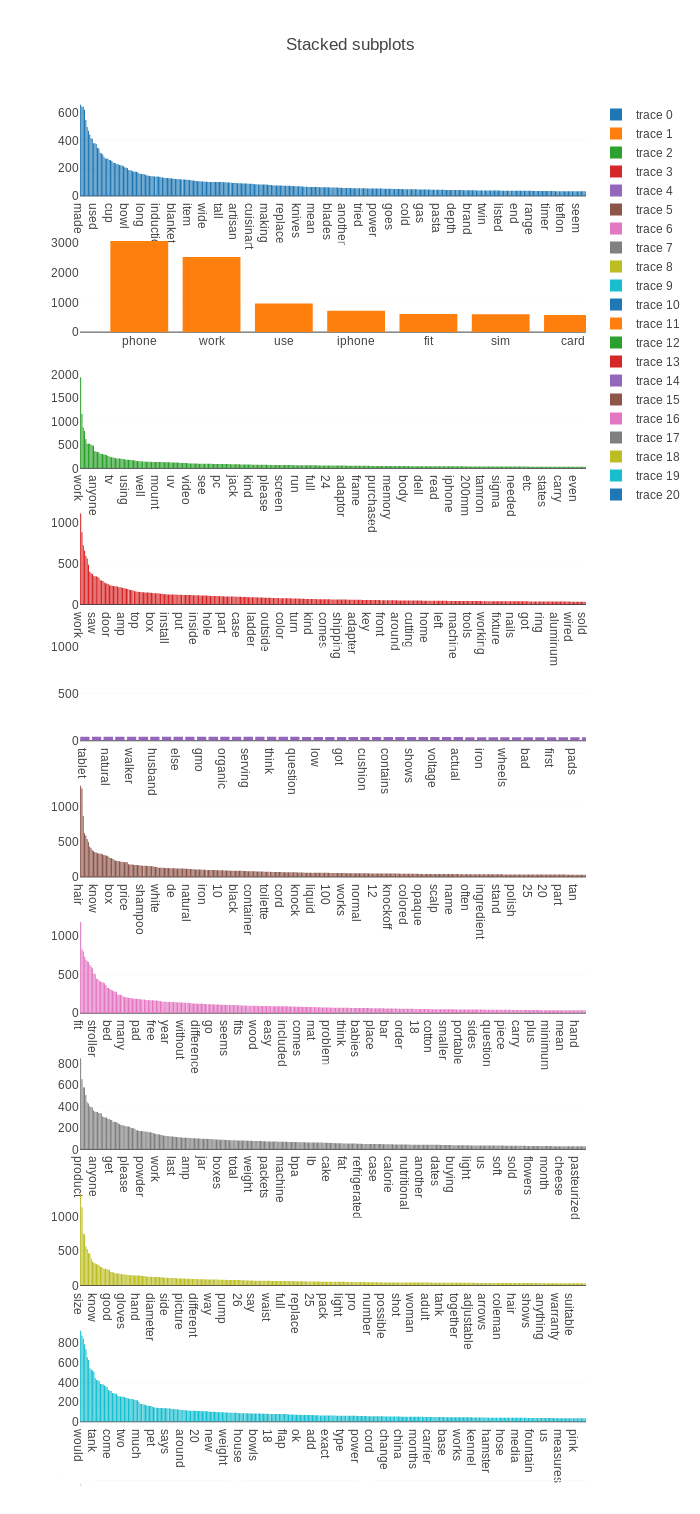
\includegraphics[width=0.7\textwidth]{pictures/words0.png}\\[3ex]
\caption{A tree of chunks of a sentence}
\label{fig:chunktree}
\end{figure}

\begin{figure}
\centering
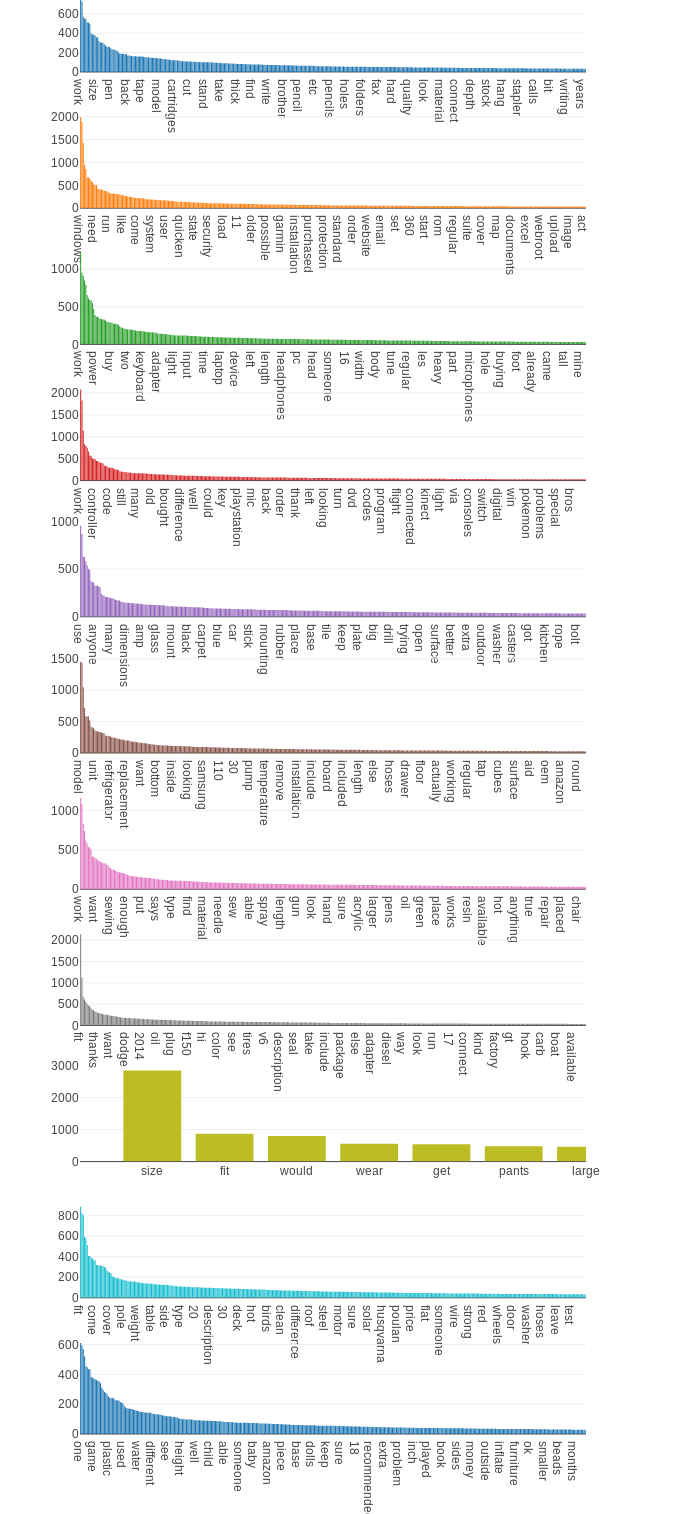
\includegraphics[width=0.7\textwidth]{pictures/words1.png}\\[3ex]
\caption{A tree of chunks of a sentence}
\label{fig:chunktree}
\end{figure}

\section{Reviews}
[better]
\begin{itemize}
   \item Information extraction systems search large bodies of unrestricted text for specific types of entities and relations, and use them to populate well-organized databases. These databases can then be used to find answers for specific questions.
   \item The typical architecture for an information extraction system begins by segmenting, tokenizing, and part-of-speech tagging the text. 
   \item The resulting data is then searched for specific types of entity. Finally, the information extraction system looks at entities that are mentioned near one another in the text, and tries to determine whether specific relationships hold between those entities.
   \item Entity recognition is often performed using chunkers, which segment multi-token sequences, and label them with the appropriate entity type. Common entity types include ORGANIZATION, PERSON, LOCATION, DATE, TIME, MONEY, and GPE (geo-political entity).
   \item Chunkers can be constructed using rule-based systems, such as the RegexpParser class provided by NLTK; or using machine learning techniques. In either case, part-of-speech tags are often a very important feature when searching for chunks.
   \item Although chunkers are specialized to create relatively flat data structures, where no two chunks are allowed to overlap, they can be cascaded together to build nested structures.
   \item Relation extraction can be performed using either rule-based systems which typically look for specific patterns in the text that connect entities and the intervening words; or using machine-learning systems which typically attempt to learn such patterns automatically from a training corpus.
\end{itemize}

\subsection{Sentence structure}

\begin{figure}
\centering
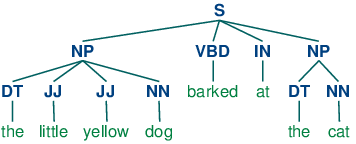
\includegraphics[width=0.7\textwidth]{pictures/chunktree.png}\\[3ex]
\caption{A tree of chunks of a sentence}
\label{fig:chunktree}
\end{figure}

\subsection{Subjects, verbs and objects}

\subsection{Relations}

\chapter{Ontology extraction and population}

The idea of the whole project was to make data collected from product pages on the marketplace - any kind of data present on the page, from the product details that are directly provided by the vendor, like size and color of an item, to data present in user generated text, namely reviews and questions/answers.

The data collected from the analysis is composed by different data types, classes of items and relationships between them.

As defined in [Gruber, 1993] \cite{gruber_translation_1993}, 
\begin{quote}
A specification of a representational vocabulary for a shared domain of discourse — definitions of classes, relations, functions, and other objects — is called an ontology. 
\end{quote}

An ontology is perfectly apt to describe, in a human-readable and useful for [being interpreted by a computer] data and relationships between data.

\section{Ontologies}
[better]
The main aim of ontology is to provide knowledge about specific domains that are understandable
by both the computers and developers. It also helps to interpret a text review at a finger
granularity with shared meanings and provides a sound semantic ground of machine-
understandable description of digital content. Ontology improves the process of information retrieval and reasoning thus
results in making data interoperable between different applications (Zhou, Chaovalit, 2007)
According to Meersman(2005), most of the ontologies in the community of information
systems are known as data models that are mainly used for structuring a fairly narrow
application domain. He claimed that ontologies that includes lexicons and thesauri may be
a useful first step in providing and formalizing the semantics of information
representation. According to Meersman (2005), in near future these ontologies will act as a
semantic domain for the information systems and will be very useful.He also predicted with
authenticity that:
\begin{quote}“ It is unmistakable that with the advent of e-commerce, and the resulting natural language
context of its related activities, that ontologies, lexicons and the thesauri and research in
their use for system design and interpretation will receive a major market driven push”
\end{quote}
(Meersman,2005,p.02)
According to Meersman, (2005), a lexicon is defined as a language-specific ontology, for e.g
English, Polish. Whereas thesaurus is defined as either a domain-specific ontology or an
application specific ontology. Manufacturing, Laptop-manufacturing, Naïve physics,
corporate law, Ontology theory are examples of domain specific ontologies, whereas Inventory
Control, Airline Reservations, Conference Organization are examples of application
specific ontology. Domain specific ontology and application specific ontology can be
distinguished intuitively as the differences between the two types are not distinct. There is
difference between ontologies and conceptual schemas but both are intimately related and are
used to represent commonly perceived reality. Mathematically, ontology is the domain while
the relational schema is the range of the semantic interpretation mapping. Both can be seen as
a representation of a commonly perceived reality and intimately related.

\section{Translating the data to an OWL ontology}
[TODO]

\section{Taxonomy of classes}
[TODO]
Amazon categorizes each item in classes.

For example, the item \texttt{Trivial Pursuit Game: Classic Edition} is classified as belonging to the class \texttt{Board Games}. The class \texttt{Board Games} is a subclass of the class \texttt{Games}, which is in turn subclass of \texttt{Toys \& Games}.

\texttt{Super Jumbo Playing Cards}, instead, are categorized as \texttt{Standard Playing Card Decks}, subclass, again, of \texttt{Games}

These classes form a tree-like hierarchical structure. 

[Amazon doesn't directly show to us how this tree is made, but we can extract it with python]

\begin{tabular}{ |l|l|l| }
\hline
\multicolumn{3}{ |c| }{Classes} \\
\hline
Depth1 & Depth2 & Depth3 \\ \hline
\multirow{4}{*}{Defenders} 
 & LB & Lucas Radebe \\
 & DC & Michael Duburry \\
 & DC & Dominic Matteo \\
 & RB & Didier Domi \\ \hline
\multirow{3}{*}{Midfielders} 
 & MC & David Batty \\
 & MC & Eirik Bakke \\
 & MC & Jody Morris \\ \hline
Forward & FW & Jamie McMaster \\ \hline
\multirow{2}{*}{Strikers} 
 & ST & Alan Smith \\
 & ST & Mark Viduka \\
\hline
\end{tabular}


\section{Populating the ontology via python}

[Populating the ontology via python has been done via the owlready library.]

\section{dataProperties and objectProperties}

In OWL, we have two possible kinds of properties that a member of the ontology can have:
\begin{itemize}
	\item DataProperty
	\item ObjectProperty
\end{itemize}

\section{Querying the ontology}

[Having an ontology like this one allows us to query the contents]
Protegé supports DL queries on the knowledge base.

\texttt{color value black and brand value Samsung}


\chapter{Results}

\section{Use cases}

\chapter{Future work}

Selection bias: users who post reviews may be a different subset than users who do not

\chapter{Conclusioni}


\backmatter
% bibliography
\cleardoublepage
\phantomsection
\bibliographystyle{sapthesis} % BibTeX style
\bibliography{/home/rana/thesis/bibliography} % BibTeX database without .bib extension

\end{document}
